\chapter{HASIL DAN PEMBAHASAN}
\label{hasil-dan-pembahasan}
Sistem bangunan yang dijadikan objek penelitian adalah \textit{climate chamber} DTNTF FT-UGM. Dalam bab ini, akan dibahas mengenai hasil perancangan kontroler sesuai dengan langkah-langkah yang dijelaskan pada Bab IV.

\section{Identifikasi Sistem}

Pada penelitian \cite{skripsiIchfan}, Kurniawan melakukan karakterisasi lingkungan termal dengan pendekatan numerik yaitu menggunakan pendekatan numerik melalui simulasi CFD. Metode yang digunakan Kurniawan yaitu dengan melakukan pemodelan kawasan \textit{climate chamber} dengan menggunakan piranti lunak IES-VE. Model yang dibangun Kurniawan divalidasi dengan hasil pengukuran di 4 titik \textit{climate chamber}. Model yang dibangun digunakan untuk memprediksi karakter lingkungan termal \textit{climate chamber} dengan memvariasikan berbagai skenario gangguan. Model IES-VE yang dibangun Kurniawan dapat mewakili variabel lingkungan termal meliputi variabel suhu dengan selisih 0,8$\pm$0,7$^\circ$C, variabel kelembapan relatif dengan selisih 2,5$\pm$3,8\%, serta variabel kecepatan udara dengan selisih 0,056$\pm$0,004 m/s. Perangkat yang paling mempengaruhi \textit{climate chamber} merupakan perangkat AC dan \textit{heater}. AC menyebabkan perubahan suhu sesuai \textit{set point}. \textit{Heater} menyebabkan perubahan suhu hingga 3,2$^\circ$C/perangkat dan kelembaban relatif 3,5\%/perangkat. Manipulasi dari AC berpengaruh besar pada variabel kecepatan udara yang menyebabkan perubahan kecepatan udara sebesar 0,9 m/s.

Pada penelitian Hartanto \cite{skripsiTanto}, model IES-VE yang telah dibangun Kurniawan digunakan untuk memperoleh data lingkungan termal. Sampel data yang digunakan sebanyak 24.000 data. Data tersebut digunakan untuk membangun model \textit{plant} lingkungan termal sistem \textit{climate chamber} menggunakan jaringan saraf tiruan. Jaringan dengan model terpilih menghasilkan MAE antara target dengan prediksi suhu sebesar 0,59$^\circ$C. Sedangkan antara target dan prediksi kelembapan relatif sebesar 5,44\%. Akurasi jaringan terpilih sebesar 96,23\% untuk suhu udara dan 68,90\% untuk kelembaban relatif.

Pada penelitian ini, digunakan model IES-VE yang dibangun Kurniawan untuk memperoleh data lingkungan termal \textit{climate chamber} bersamaan dengan Hartanto. Kemudian, model yang dibangun Hartanto digunakan dalam penelitian ini sebagai model \textit{plant} dalam proses simulasi.

\subsection{Pengambilan Data Simulasi IES-VE}

Pada Gambar \ref{fig:4:HasilSimulasiIESVE} ditunjukkan salah satu hasil simulasi untuk skenario AC 26$^\circ$C dan \textit{heater} ON 2 buah dengan variabel gangguan yang digambarkan pada Gambar \ref{fig:4:LoadSimulasiIESVE}. Grafik yang ditampilkan terdiri dari 4 parameter yaitu suhu lingkungan (T$_o$), intensitas radiasi matahari (RD), suhu ruang (T$_{db}$), dan kelembapan relatif (RH). Skenario ini dilakukan selama 24 jam dengan selang waktu pengambilan data selama 6 menit dimulai dari pukul 00:03 hingga 23:57 WIB. Selang waktu tersebut adalah waktu tersingkat yang dapat dilakukan pada software IES-VE 2019. Respon waktu suhu ruang terhadap aktivasi AC tidak diperhitungkan dikarenakan secara fisis, respons transien termal pada bangunan berlangsung cukup lama, sehingga hanya berfokus untuk meninjau nilai \textit{steady-state error}.

\begin{figure}[!h]
	\centering
	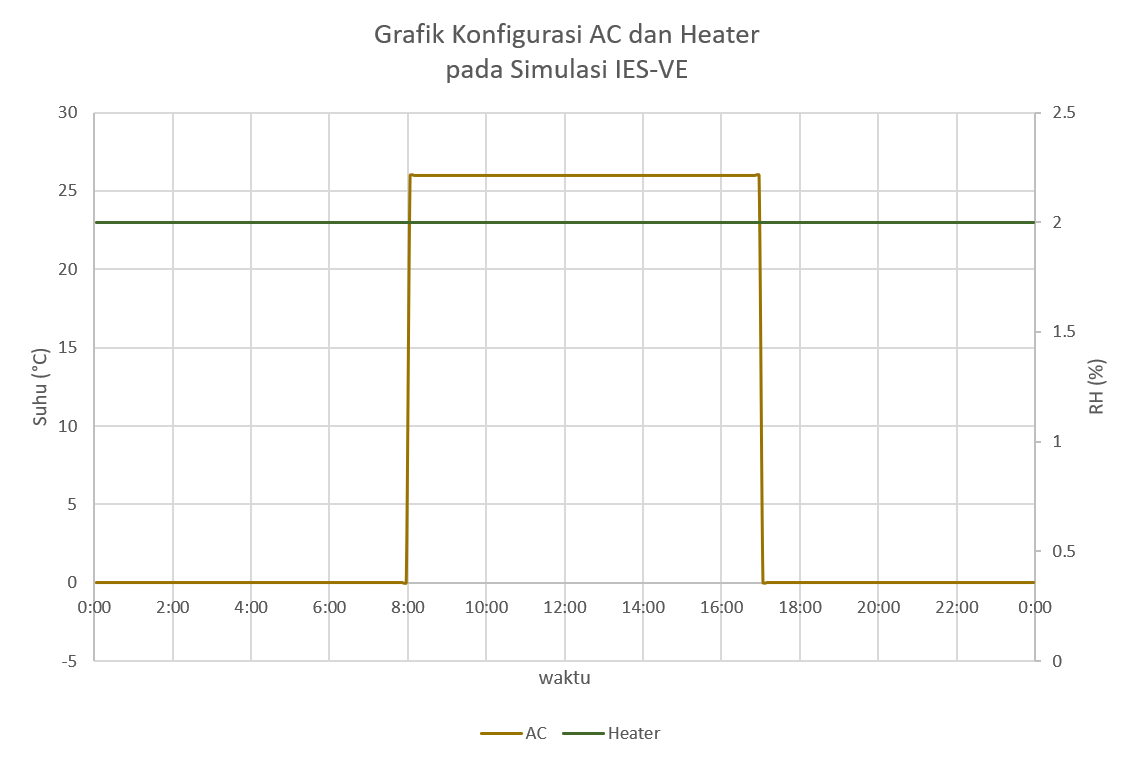
\includegraphics[width=1\textwidth]{figures/ACHTSimulasiIESVE}
	\caption{Data Konfigurasi AC dan \textit{Heater} pada Simulasi ISE-VE}
	\label{fig:4:ACHTSimulasiIESVE}
\end{figure}
\vspace{1em}

\begin{figure}[!h]
	\centering
	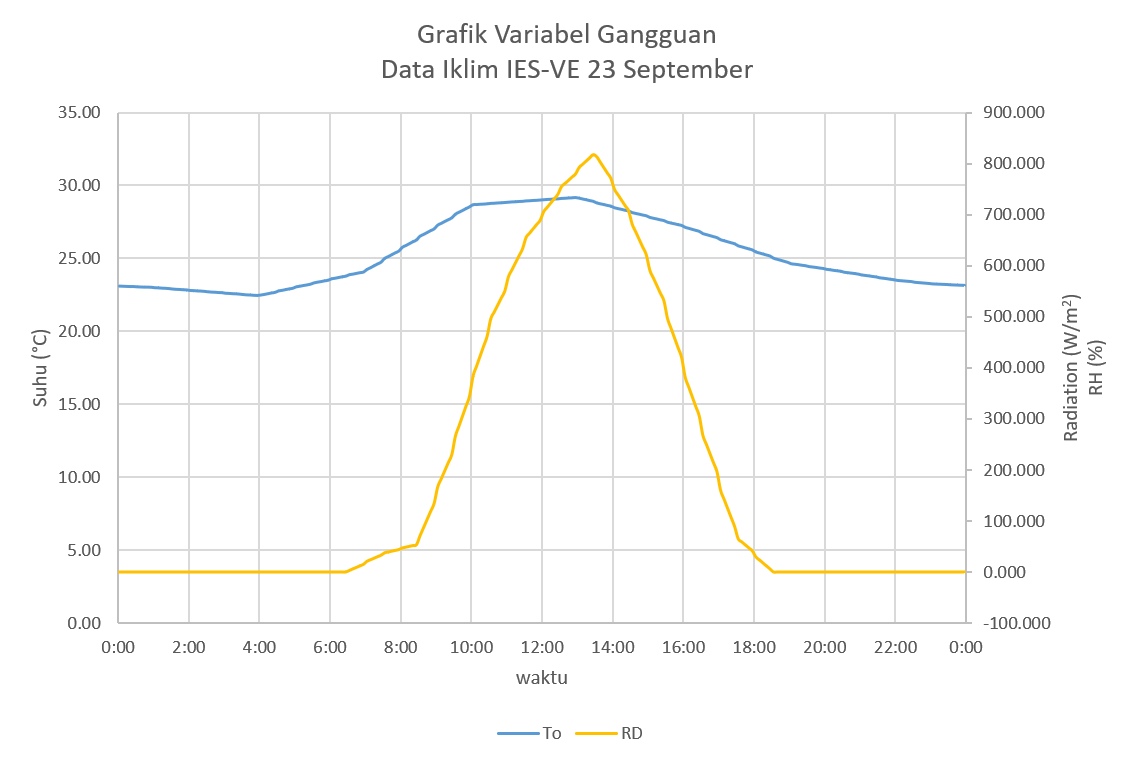
\includegraphics[width=1\textwidth]{figures/LoadSimulasiIESVE}
	\caption{Variabel Gangguan Simulasi ISE-VE}
	\label{fig:4:LoadSimulasiIESVE}
\end{figure}
\vspace{1em}
\hfill\break

\begin{figure}[!h]
	\centering
	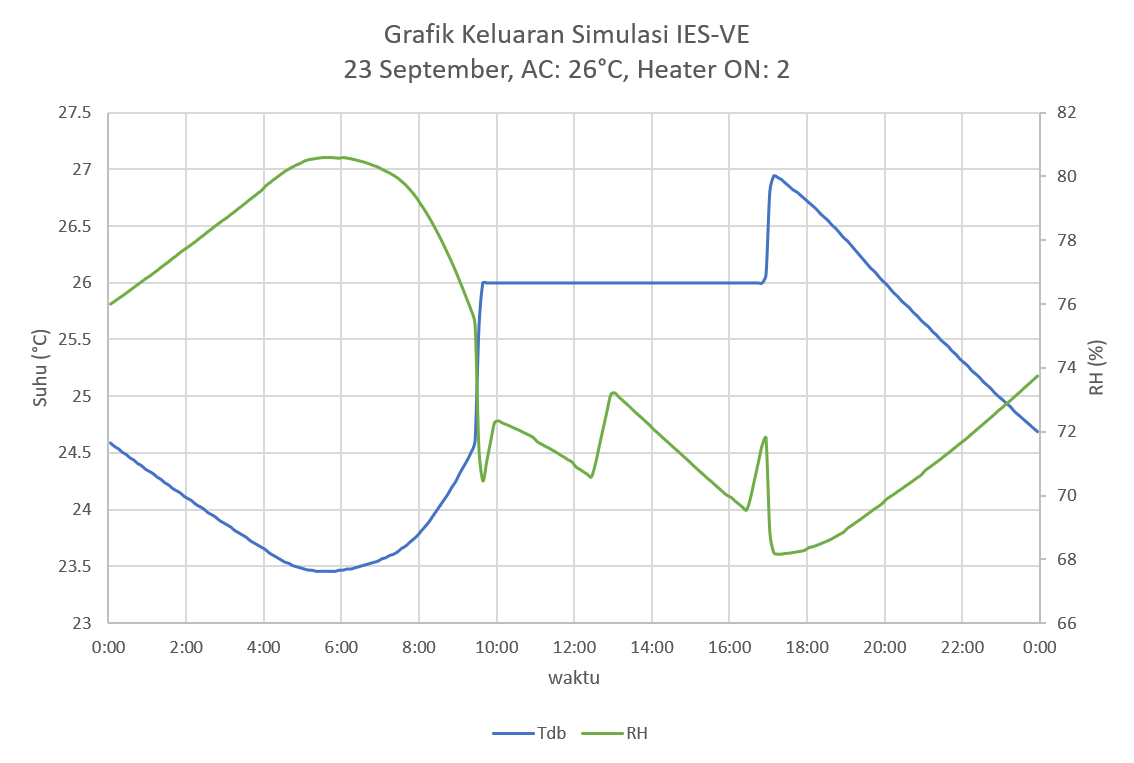
\includegraphics[width=1\textwidth]{figures/HasilSimulasiIESVE}
	\caption{Data Hasil Simulasi ISE-VE}
	\label{fig:4:HasilSimulasiIESVE}
\end{figure}
\vspace{1em}
\break

\subsection{Identifikasi Sistem Pengendalian}

Dalam perancangan sistem kendali, perlu diidentifikasi terlebih dahulu variabel-variabel yang terlibat pada suatu sistem. Terdapat beberapa variabel yang terlibat pada sistem \textit{climate chamber}. Variabel-variabel yang diangkat pada penelitian ini tunjukkan oleh diagram blok \textit{plant} pada Gambar \ref{fig:5:DiagramBlokPlant}. Berdasarkan diagram tersebut, dapat dikatakan bahwa sistem merupakan sistem MIMO (\textit{Multi Input Multi Output}) yaitu sistem yang memiliki beberapa masukan dan beberapa keluaran. Identifikasi sistem yang telah dilakukan akan menghasilkan suatu diagram blok fungsional sistem seperti yang ditunjukkan pada Gambar \ref{fig:5:DiagramBlokSistem}.

\begin{figure}[!h]
	\centering
	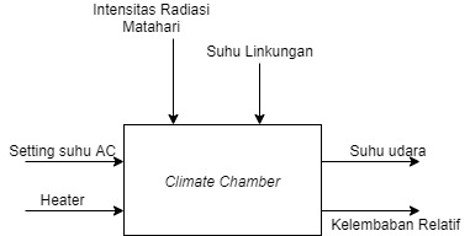
\includegraphics[width=0.55\textwidth]{figures/BlokDiagramPlant}
	\caption{Diagram Blok \textit{Plant}}
	\label{fig:5:DiagramBlokPlant}
\end{figure}
\vspace{1em}

Dalam sistem \textit{climate chamber}, variabel manipulasi yang digunakan adalah \textit{setting} suhu AC dan \textit{heater} (jumlah \textit{heater} ON). Kemudian, variabel kontrol yang digunakan yaitu suhu udara (T$_{db}$) dan kelembapan relatif (RH) pada \textit{plant} (\textit{climate chamber}). Ada pula variabel gangguan sistem yaitu berupa intensitas radiasi matahari dan suhu lingkungan. Perubahan suhu oleh AC hanya mampu bekerja dengan kenaikan nilai sebesar 1$^\circ$C. Dengan memperhatikan \textit{manipulator} (\textit{final control elements}) yang digunakan, secara fisis RH tidaklah mungkin dapat dikendalikan oleh kontroler. Perubahan nilai RH yang terjadi diakibatkan oleh pengaruh AC secara tidak langsung. Untuk pengujian \textit{set point}, skenario pengujian mengadaptasi Tugas Akhir pengujian level sensasi termal yang dilakukan oleh Nadiya\cite{skripsiMuna}. Hanya saja pada penelitian menggunakan \textit{set point} step bertingkat dengan lompatan 2$^{\circ}$C dari nilai suhu sebesar 16$^{\circ}$C hingga 30$^{\circ}$C.

\begin{figure}[!h]
	\centering
	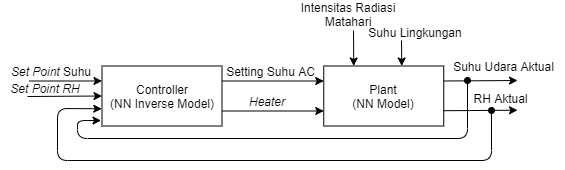
\includegraphics[width=0.85\textwidth]{figures/DiagramBlokFungsionalSistem}
	\caption{Diagram Blok Fungsional Sistem}
	\label{fig:5:DiagramBlokSistem}
\end{figure}

Kontroler pada \textit{climate chamber} memiliki enam buah variabel masukan dan dua buah variabel keluaran. Variabel masukan kendali ini yaitu nilai \textit{set point} suhu udara, \textit{set point} kelembapan relatif, nilai aktual umpan balik suhu udara, nilai aktual umpan balik kelembapan relatif, nilai umpan balik \textit{setting} suhu AC, dan nilai umpan balik \textit{heater}. Sementara, variabel keluaran kontroler ini adalah \textit{setting} suhu AC dan \textit{heater} (jumlah \textit{heater} ON).

Untuk memaksimalkan kinerja kontroler, pada proses pelatihan JST (kontroler) dilakukan penskalaan terhadap semua variabel masukan JST menggunakan metode \textit{Min Max Scaling} kecuali variabel umpan balik \textit{setting} suhu AC dan variabel umpan balik \textit{heater}. Penskalaan bertujuan untuk meningkatkan kinerja JST menjadi optimal dengan menyamakan rentang nilai dan besar satuan dari setiap variabel (berupa rentang nilai dari 0 hingga 1). Masing-masing variabel diubah menjadi skala satuan dengan melakukan transformasi data secara statistik. Data dari setiap variabel akan dikurangi dengan nilai minimum variabel tersebut yang dikemudian dibagi oleh selisih dari nilai maksimum dan nilai minimum variabel tersebut. Dengan demikian, ditambahkan pula blok \textit{scaler} pada diagram blok sistem kontrol agar nilai masukan kontroler dapat disesuaikan.

\begin{figure}[!h]
	\centering
	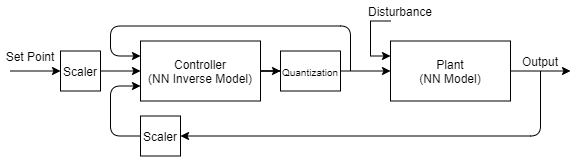
\includegraphics[width=0.85\textwidth]{figures/ControlDesignDiagramII}
	\caption{Diagram blok sistem kontrol berbasis JST}
	\label{fig:5:ConstrolSystemBlockDiagram}
\end{figure}

Diagram blok sistem kontrol juga memiliki blok tambahan berupa blok kuantisasi (\textit{Quantization}). Blok ini berperan sebagai penyesuai nilai variabel manipulasi yang dihasilkan kontroler. Hal ini dilakukan karena pada praktiknya nilai \textit{setting} suhu AC merupakan nilai bilangan bulat dan bukan nilai bilangan desimal. Hal ini pun berlaku untuk variabel manipulasi \textit{heater} di mana nilainya berupa nilai 0, 1, atau 2 yang menunjukkan jumlah \textit{heater} ON/menyala. Sehingga tidak mungkin ada nilai diantara nilai tersebut. Dengan demikian, diagram blok dipasangi sebuah blok kuantisasi (\textit{Quantization}) yang berfungsi untuk menghindari nilai desimal atau pun nilai yang berada di luar rentang nilai variabel manipulasi. Pada akhirnya dihasilkan diagram blok sistem kontrol yang ditunjukkan pada Gambar \ref{fig:5:ConstrolSystemBlockDiagram}.

\section{Rancangan Kontrol berbasis JST}

Model JST kontroler dibangun dengan menggunakan model jaringan saraf tiruan arsitektur \textit{feedforward neural network} dengan 1 lapisan tersembunyi. Pada Sub Bab ini akan dijabarkan hasil dari proses perancangan model JST untuk kontroler.

\subsection{Variasi Pembagian Data Perancangan JST Kontroler}

Dalam memvariasikan pembagian data digunakan metode \textit{trial-and-error} berdasarkan artikel \cite{DataSplitting}. Pada penelitian ini, variasi pembagiaan data dilakukan dengan membandingkan beberapa variasi pembagiaan data ke dalam 5 variasi. Kemudian kinerja dari setiap pembagian data dibandingkan dengan konfigurasi \textit{hyperparameter} pada Tabel \ref{tbl:5:NeuronVariation}.

\begin{table}[!h]
	\caption{Tabel Daftar Variasi Pembagian Data}
	\label{tbl:5:NeuronVariation}
	\centering
	% use packages: array
	\begin{tabular}{|p{3.2cm}|p{3cm}|}
		\hline
		\textbf{Pembagian Data} & \textbf{Persentase Data} \\ \hline
		Pembagian Data 1 & (50\% 25\% 25\%) \\ \hline
		Pembagian Data 2 & (60\% 20\% 20\%) \\ \hline
		Pembagian Data 3 & (70\% 15\% 15\%) \\ \hline
		Pembagian Data 4 & (80\% 10\% 10\%) \\ \hline
		Pembagian Data 5 & (80\% 15\% 05\%) \\ \hline
	\end{tabular}
\end{table}

Model JST untuk membandingkan variasi pembagian data menggunakan arsitektur \textit{feedforward network} dengan 1 lapisan tersembunyi berisi 10 neuron. Pada tabel yang disajikan, pembagian data ditulis dengan format "Pembagian Data n" dan "(x\% y\% z\%)" di mana n = nomor variasi, x = pembagian data pelatihan, y = pembagian data validasi, dan z = pembagian data pengujian. Berdasarkan hasil variasi yang ditunjukkan pada Gambar \ref{fig:5:DataSplittingVariation}, didapatkan pembagian data terbaik yaitu pembagian data bernama "Pembagian Data 4". Data dibagi menjadi 3 bagian, yakni 80\% data pelatihan, 10\% data validasi, dan 10\% data pengujian.

\begin{figure}[!h]
	\centering
	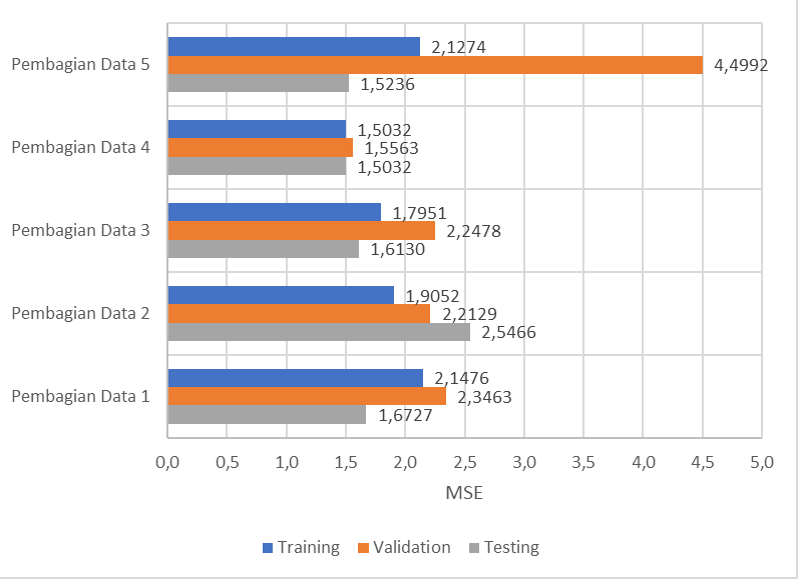
\includegraphics[width=0.85\textwidth]{figures/VariasiPembagianDataJSTKontroler}
	\caption{Grafik Variasi Pembagian Data}
	\label{fig:5:DataSplittingVariation}
\end{figure}

\subsection{Variasi Arsitektur Perancangan JST Kontroler}

Pada perancangan model JST kontroler digunakan 2 variasi fungsi aktivasi, yaitu fungsi tansig (fungsi \textit{hyperbolic tanget}) dan fungsi logsig (fungsi sigmoid). Kemudian masing-masing dilatih dengan jumlah neuron yang bervariasi dari 5 neuron hingga 60 neuron dengan lompatan sebesar 5 neuron. Dari proses variasi ini, didapatkan hasil bahwa model yang menggunakan fungsi aktivasi tansig dengan 35 neuron menghasilkan kinerja dengan nilai MSE terkecil. Hasil dari variasi ini ditunjukkan pada Gambar \ref{fig:5:ActivationVariation}.

\begin{figure}[!h]
	\centering
	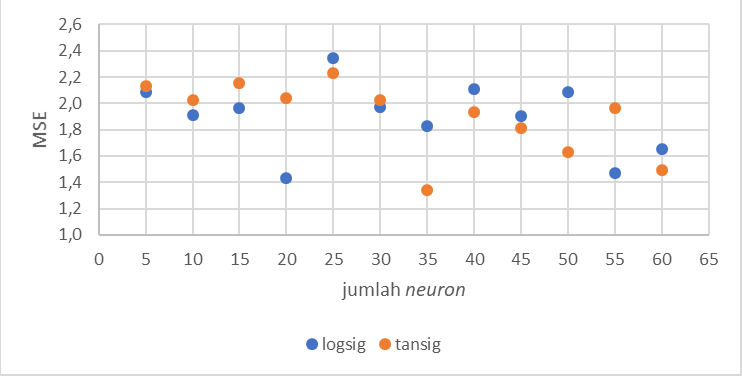
\includegraphics[width=0.75\textwidth]{figures/ActivationVariation}
	\caption{Grafik Persebaran MSE Variasi Arsitektur JST Kontroler}
	\label{fig:5:ActivationVariation}
\end{figure}

Kemudian arsitektur JST divariasikan kembali menggunakan fungsi aktivasi tansig dari 30 neuron hingga 40 neuron dengan lompatan sebesar 1 neuron untuk mengetahui kinerja model pada jumlah neuron yang berdekatan. Setelah dilakukan variasi, didapatkan hasil bahwa model JST dengan 35 neuron masih merupakan model arsitektur terbaik dengan nilai MSE terkecil. Hasil variasi ini dapat dilihat pada Gambar \ref{fig:5:NeuronVariation}.

\begin{figure}[!h]
	\centering
	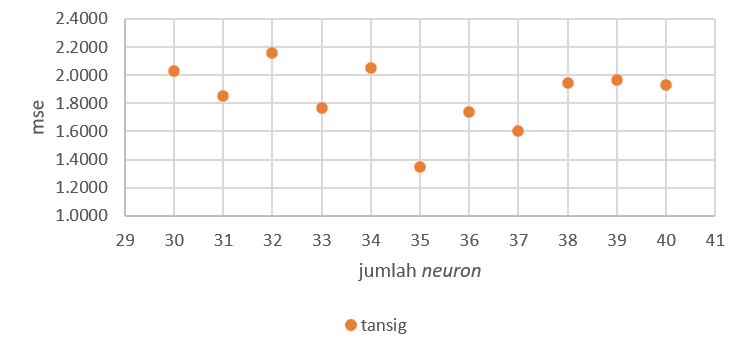
\includegraphics[width=0.75\textwidth]{figures/NeuronVariation}
	\caption{Grafik Persebaran MSE Variasi Arsitektur JST Kontroler}
	\label{fig:5:NeuronVariation}
\end{figure}

\subsection{Hasil Rancangan Model JST Kontroler}

Setelah dilakukan perancangan model JST melalui variasi arsitektur model, didapatkan rancangan model JST kontroler terbaik. Model JST dibangun dengan arsitektur \textit{feedforward neural network} 1 lapisan tersembunyi dengan 35 neuron. Model JST menggunakan fungsi aktivasi tansig (\textit{hyperbolic tanget}) dan algoritma pembelajaran Levenberg-Marquardt. Model JST Kontroler terbaik memiliki nilai \textit{hyperparameter} yang diringkas pada Tabel \ref{tbl:5:NNControl}.
 
\begin{table}[!h]
	\caption{Tabel Rancangan Kontroler JST (\textit{NN Inverse Model})}
	\label{tbl:5:NNControl}
	\centering
	% use packages: array
	\begin{tabular}{|p{5.7cm}|p{6.5cm}|}
		\hline
		\textbf{Nama Hyperparameter} & \textbf{Nilai Hyperparameter} \\ \hline
		Arsitektur & Feedforward Neural Network \\ \hline
		Pembagian Data & 80\% 10\% 10\% \\ \hline 
		Jumlah Layar Tersembunyi & 1 \\ \hline
		Jumlah Neuron pada Layar & [35] \\ \hline
		Fungsi Aktivasi Layar & Hyperbolic Tangent (tansig) \\ \hline
		Algoritma Pembelajaran & Levenberg-Marquardt \\ \hline
		Mean Absolute Error (MAE) & AC: 0,37$^\circ$C ; HT: 0,02 Perangkat ON\\ \hline
		Mean Squared Error (MSE) & AC: 2,68$^\circ$C ; HT: 0,01 Perangkat ON\\ \hline
		Koefisien Korelasi (R) & AC: 99,12\% ; HT: 99,65\% \\ \hline
	\end{tabular}
\end{table}

Model JST Kontroler memiliki nilai MAE sebesar 0,37$^\circ$C di mana nilai ini di bawah 1$^\circ$C. Dengan demikian, model JST dapat digunakan sebagai model kontroler. Model hasil rancangan ini kemudian diubah ke dalam bentuk blok SIMULINK dengan menggunakan perintah \textit{gensim} yang kemudian akan dijadikan blok kontroler untuk simulasi sistem kontrol pada SIMULINK.

\section{Hasil Simulasi Kontrol SIMULINK}

Pada simulasi kontrol, digunakan nilai \textit{set point} sesuai dengan uji eksperimental level sensasi termal yang dilakukan oleh Nadiya pada \textit{climate chamber} \cite{skripsiMuna}. Perbedaannya, pada penelitian ini variasi naik turun suhu dari 16$^\circ$C hingga 30$^\circ$C menggunakan lompatan sebesar 2$^\circ$C.

\subsection{Skenario Pemanasan Pendinginan dengan Variabel Gangguan Konstan}

Pada simulasi ini digunakan nilai variabel gangguan konstan sebesar 26,8$^\circ$C untuk suhu lingkungan dan 423,343 $W/m^2$ untuk intensitas radiasi matahari. Nilai-nilai variabel gangguan tersebut merupakan nilai rerata dari variabel gangguan pada jam operasi penggunaan \textit{climate chamber}, yaitu pukul 08:00 WIB sampai dengan pukul 17:00 WIB. Berdasarkan hasil simulasi, kontroler mampu mengendalikan suhu ruang dan kelembapan relatif mengikuti nilai \textit{set point}. Akan tetapi, kontroler tidak mampu menaikan suhu ruang mencapai nilai lebih dari 27$^\circ$C. Hal ini terjadi diakibatkan kontroler gagal dalam mengaktifkan 2 \textit{heater} disaat nilai \textit{setting} AC tidak mampu melebihi nilai maksimum (SET 30$^\circ$C). Kombinasi \textit{set point} dan hasil simulasi ditunjukkan pada Gambar \ref{fig:5:SimulinkTd} dan Gambar \ref{fig:5:SimulinkRH}.

\begin{figure}[!h]
	\centering
	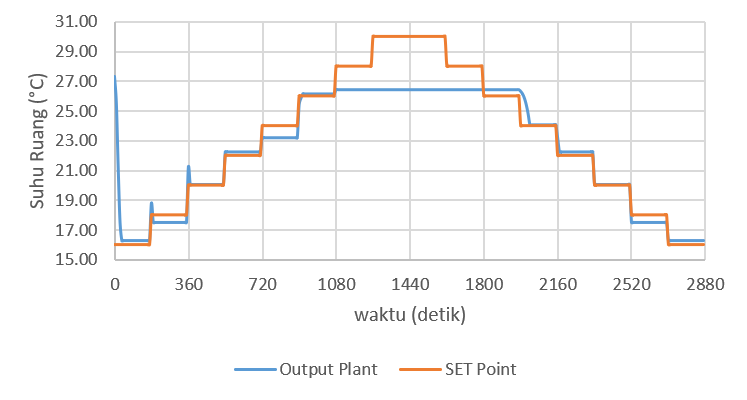
\includegraphics[width=0.75\textwidth]{figures/Simulink1Td}
	\caption{Grafik Hasil Simulasi 1 Simulink untuk Suhu Ruang}
	\label{fig:5:SimulinkTd}
\end{figure}

\begin{figure}[!h]
	\centering
	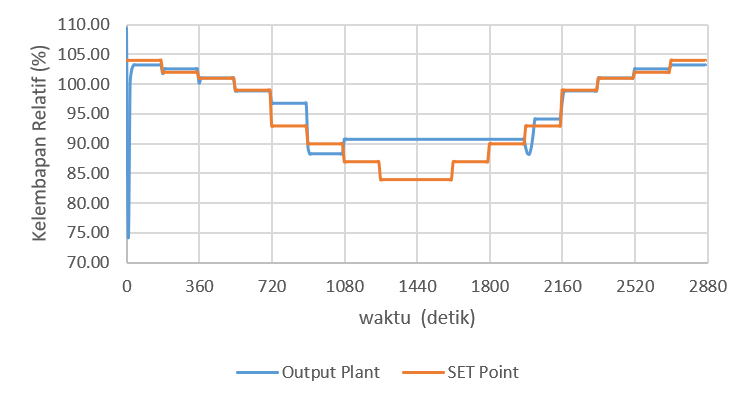
\includegraphics[width=0.75\textwidth]{figures/Simulink1RH}
	\caption{Grafik Hasil Simulasi 1 Simulink untuk Kelembapan Relatif}
	\label{fig:5:SimulinkRH}
\end{figure}

\begin{figure}[!h]
	\centering
	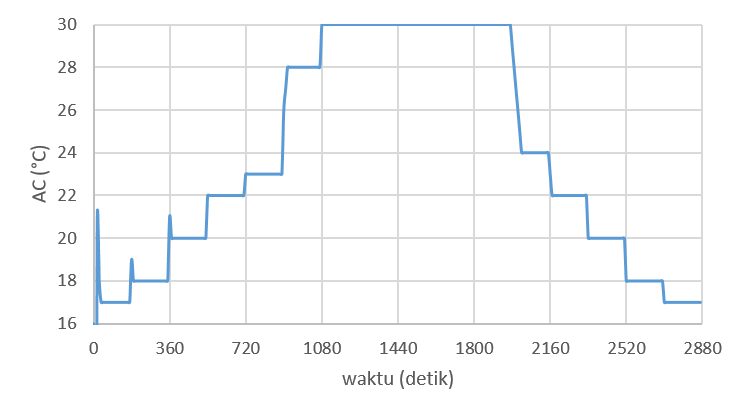
\includegraphics[width=0.75\textwidth]{figures/Simulink1AC}
	\caption{Grafik Variabel Manipulasi AC pada Simulasi 1 Simulink}
	\label{fig:5:SimulinkAC}
\end{figure}

\begin{figure}[!h]
	\centering
	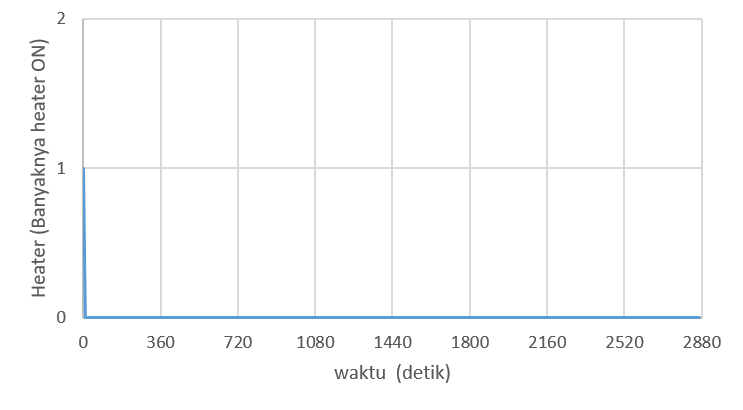
\includegraphics[width=0.75\textwidth]{figures/Simulink1HT}
	\caption{Grafik Variabel Manipulasi \textit{Heater} pada Simulasi 1 Simulink}
	\label{fig:5:SimulinkHT}
\end{figure}
\vspace{1em}

Dengan meninjau nilai variabel manipulasi AC yang ditunjukkan pada Gambar \ref{fig:5:SimulinkAC}, dapat dilihat bahwa untuk mengendalikan suhu mencapai \textit{set point} 26$^\circ$C, perangkat AC perlu mengeluarkan sinyal sebesar 28$^\circ$C (waktu ke-100 hingga ke-120). Dengan demikian, ketika \textit{set point} bernilai 28$^\circ$C, perangkat AC hanya mampu mengeluarkan sinyal maksimum 30$^\circ$C (waktu ke-120 hingga ke-140).

Kurangnya keandalan kinerja kontroler pada penelitian ini untuk mengendalikan suhu ruang di atas \textit{set point} 26$^\circ$C disebabkan oleh salah satu kelemahan model JST dalam pemodelan \textit{plant}. Secara fisis, proses pemanasan pada sistem bangunan (dalam hal ini \textit{climate chamber}) membutuhkan waktu yang cukup lama. Dengan demikian, proses pemanasan pada kenyataannya tetap bisa mencapai \textit{set point} suhu di atas 26$^\circ$C. Hanya saja proses tersebut membutuhkan waktu (\textit{settling time}) yang cukup lama. Akan tetapi, proses tersebut tidak dapat disimulasikan secara sempurna pada penelitian ini dikarenakan model JST \textit{plant} yang dibangun oleh Hartanto\cite{skripsiTanto} hanya berupa model pasangan data dan bukan berupa model yang bergantung terhadap waktu. Sehingga, model JST \textit{plant} hanya dapat langsung mengeluarkan suatu nilai keluaran setiap menerima nilai masukan.

Ditinjau dari \textit{set point} 16$^\circ$C hingga 26$^\circ$C, didapatkan nilai \textit{steady-state error} untuk suhu ruang sebesar 0,15$^\circ$C pada proses pemanasan dan sebesar 0,2$^\circ$C pada proses pendinginan. Lalu, didapatkan pula nilai \textit{steady-state error} untuk kelembapan relatif sebesar 0,05\% pada proses pemanasan dan sebesar 0,02\% pada proses pendinginan. Sehingga rerata nilai \textit{steady-state error} sebesar 0,18$^\circ$C untuk suhu ruang dan sebesar 0,04\% untuk kelembapan relatif.

\subsection{Skenario Pemanasan Pendinginan dengan Variabel Gangguan Bergerak}

Pada skenario ini digunakan data variabel gangguan pada 21 Juni 2019 yang bergerak dari pukul 08:03 sampai dengan 08:51 WIB. Nilai dari variabel gangguan ditunjukkan pada Gambar \ref{fig:5:Simulink2To} untuk suhu lingkungan dan \ref{fig:5:Simulink2RD} untuk intensitas radiasi matahari. Pada skenario ini, nilai \textit{set point} yang digunakan senilai dengan nilai \textit{set point} pada simulasi dengan variabel gangguan konstan.

\begin{figure}[!h]
	\centering
	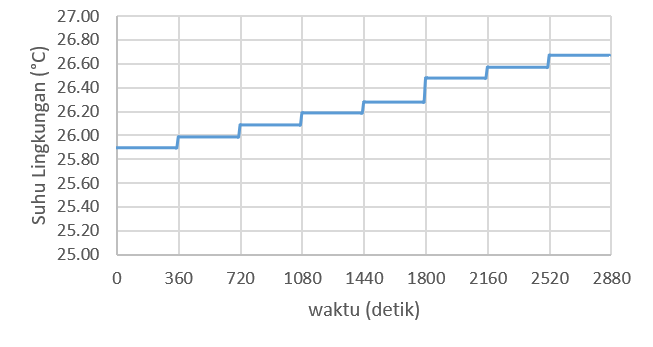
\includegraphics[width=0.7\textwidth]{figures/Simulink2To}
	\caption{Grafik Nilai Variabel Gangguan Suhu Lingkungan}
	\label{fig:5:Simulink2To}
\end{figure}

\begin{figure}[!h]
	\centering
	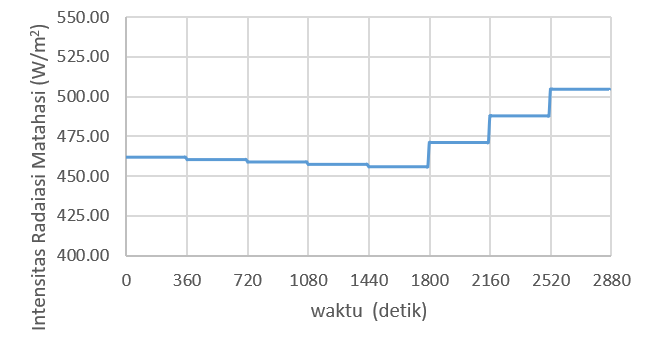
\includegraphics[width=0.7\textwidth]{figures/Simulink2RD}
	\caption{Grafik Nilai Variabel Gangguan Intensitas Radiasi Matahari}
	\label{fig:5:Simulink2RD}
\end{figure}

\begin{figure}[!h]
	\centering
	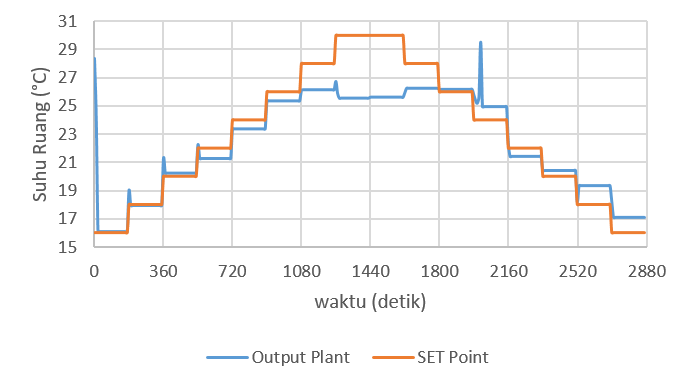
\includegraphics[width=0.7\textwidth]{figures/Simulink2Td}
	\caption{Grafik Hasil Simulasi 2 Simulink untuk Suhu Ruang}
	\label{fig:5:Simulink2Td}
\end{figure}

\begin{figure}[!h]
	\centering
	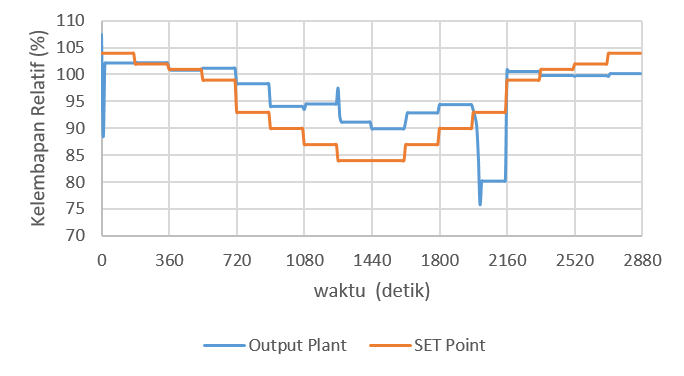
\includegraphics[width=0.7\textwidth]{figures/Simulink2RH}
	\caption{Grafik Hasil Simulasi 2 Simulink untuk Kelembapan Relatif}
	\label{fig:5:Simulink2RH}
\end{figure}

Hasil simulasi dengan variabel gangguan bergerak pun menunjukan kinerja yang kurang optimal. Berdasarkan Gambar \ref{fig:5:Simulink2Td}, dapat dilihat bahwa kontroler tidak mampu menaikan suhu ruang mencapai nilai lebih dari 27$^\circ$C. Dapat dilihat pula bahwa terjadi lonjakan nilai suhu udara pada detik ke-1980. Lonjakan tersebut terjadi akibat penonaktifan AC yang dilakukan oleh kontroler yang dapat dilihat pada Gambar \ref{fig:5:Simulink2AC}. Pada proses pendinginan, nilai \textit{steady-state error} tampak lebih besar dibandingkan saat proses pemanasan. Hal ini mungkin disebabkan karena kenaikan suhu lingkungan dan intensitas radiasi matahari. Walaupun nilai galat membesar, dapat dilihat bahwa pada proses pendinginan kontroler tetap berupaya untuk mengikuti perubahan \textit{set point}.

\begin{figure}[!h]
	\centering
	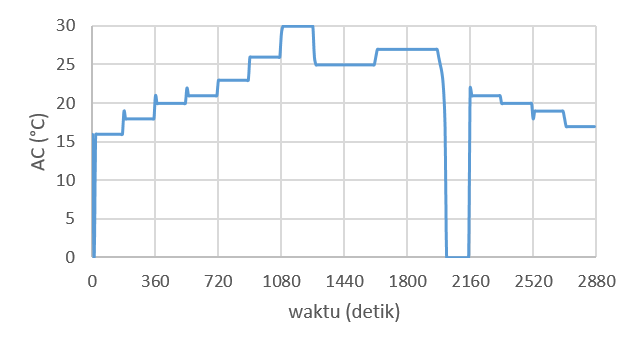
\includegraphics[width=0.65\textwidth]{figures/Simulink2AC}
	\caption{Grafik Variabel Manipulasi AC pada Simulasi 2 Simulink}
	\label{fig:5:Simulink2AC}
\end{figure}

\begin{figure}[!h]
	\centering
	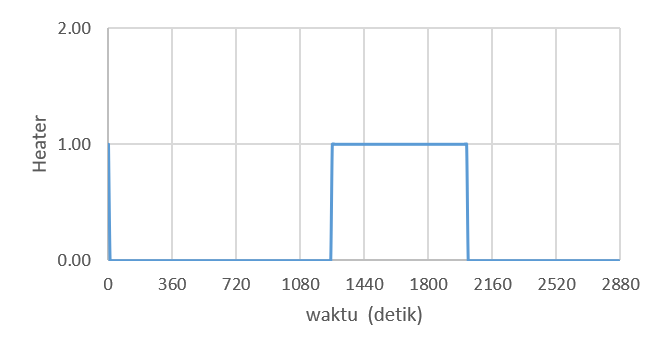
\includegraphics[width=0.65\textwidth]{figures/Simulink2HT}
	\caption{Grafik Variabel Manipulasi \textit{Heater} pada Simulasi 2 Simulink}
	\label{fig:5:Simulink2HT}
\end{figure}
\break
\subsection{Analisis Kegagalan Kendali}

Dari hasil 2 simulasi yang telah dijabarkan, kontroler jarang sekali mengaktifkan 2 \textit{heater} bahkan disaat ingin mencapai suhu yang tinggi. Hal ini menimbulkan kecurigaan terhadap rentang kinerja JST, baik pada model kontroler maupun model \textit{plant}. Untuk mengetahui penyebab kegagalan, dilakukan kembali simulasi dimana kontroler berhasil mengaktifkan 2 perangkat \textit{heater}. Simulasi ini dilakukan dengan nilai variabel gangguan sebesar 27$^\circ$C untuk suhu lingkungan dan sebesar 600 $W/m^2$ untuk intensitas radiasi matahari. Hasil simulasi ditunjukkan pada Gambar \ref{fig:5:Simulink3Td}, Gambar \ref{fig:5:Simulink3RH}, Gambar \ref{fig:5:Simulink3AC}, dan Gambar \ref{fig:5:Simulink3HT}.

\begin{figure}[!h]
	\centering
	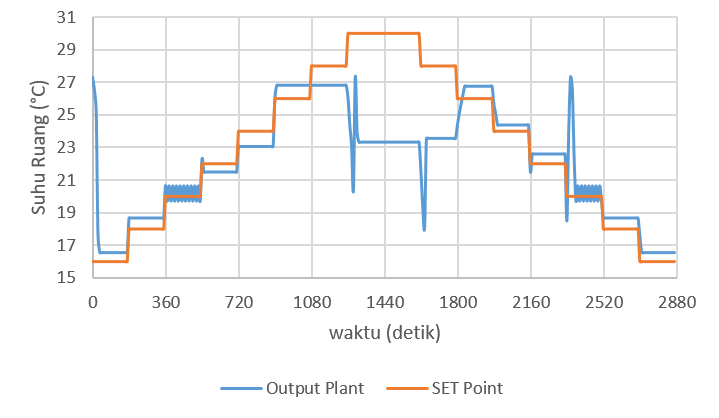
\includegraphics[width=0.65\textwidth]{figures/Simulink3Td}
	\caption{Grafik Hasil Simulasi 3 Simulink untuk Suhu Ruang}
	\label{fig:5:Simulink3Td}
\end{figure}

\begin{figure}[!h]
	\centering
	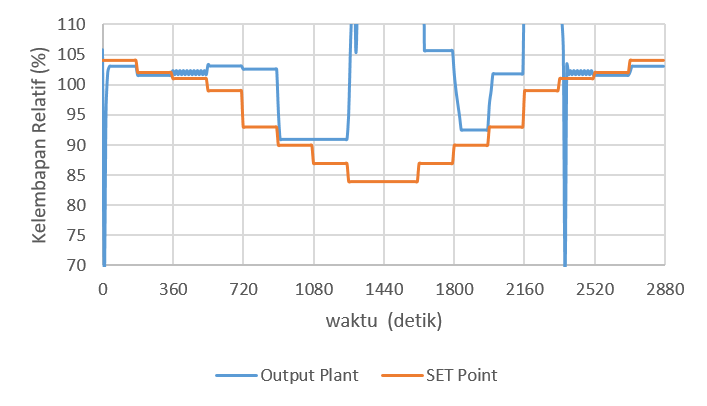
\includegraphics[width=0.65\textwidth]{figures/Simulink3RH}
	\caption{Grafik Hasil Simulasi 3 Simulink untuk Kelembapan Relatif}
	\label{fig:5:Simulink3RH}
\end{figure}

\begin{figure}[!h]
	\centering
	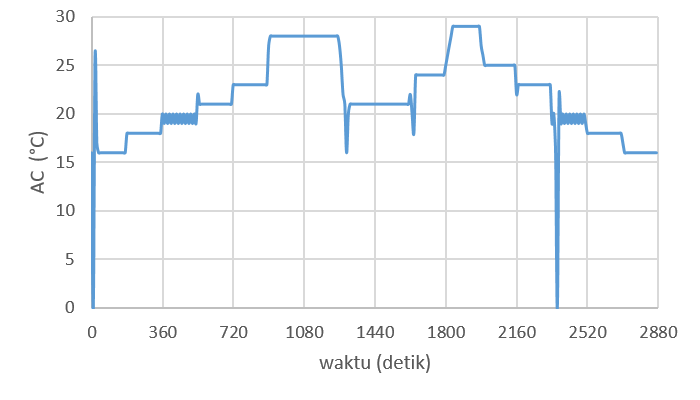
\includegraphics[width=0.75\textwidth]{figures/Simulink3AC}
	\caption{Grafik Variabel Manipulasi AC pada Simulasi 3 Simulink}
	\label{fig:5:Simulink3AC}
\end{figure}

\begin{figure}[!h]
	\centering
	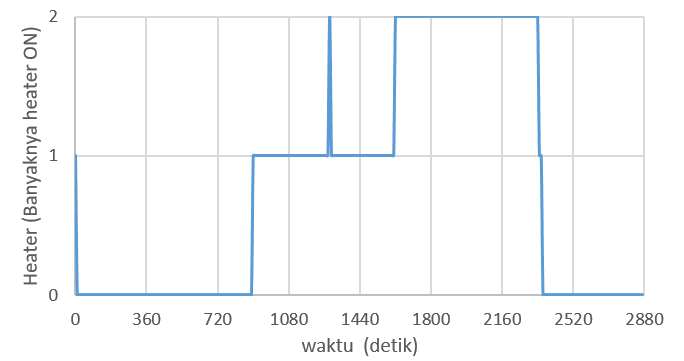
\includegraphics[width=0.65\textwidth]{figures/Simulink3HT}
	\caption{Grafik Variabel Manipulasi \textit{Heater} pada Simulasi 3 Simulink}
	\label{fig:5:Simulink3HT}
\end{figure}

Berdasarkan hasil simulasi ini, dapat disimpulkan bahwa kegagalan pengendalian bukanlah disebabkan oleh tidak aktifnya 2 buah perangkat \textit{heater}. Selanjutnya, dicoba untuk dianalis model \textit{plant} yang dibangun oleh Hartanto. Pengujian dilakuakan dengan nilai variabel gangguan yang sama dan nilai AC 30$^\circ$C serta 2 \textit{heater} ON. Grafik percobaan ditunjukkan pada Gambar \ref{fig:5:UjiPlant}\\
\break
\break
\break

\begin{figure}[!h]
	\centering
	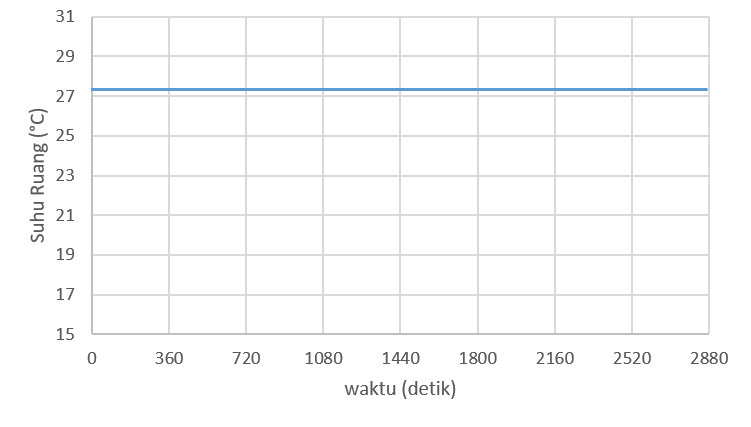
\includegraphics[width=0.75\textwidth]{figures/UjiPlant}
	\caption{Grafik Hasil Uji \textit{Plant}}
	\label{fig:5:UjiPlant}
\end{figure}
\vspace{1em}

Dari Gambar \ref{fig:5:UjiPlant} diketahui bahwa \textit{plant} memang tidak mampu untuk menghasilkan keluaran suhu diatas 28$^\circ$C. Dengan begitu, perlu ditelaah kembali mengenai data yang digunakan. Setelah diteliti, kurangnya keandalan kontroler ternyata disebabkan oleh data simulasi yang dinilai kurang cukup mewakili kondisi lingkungan termal di suhu yang tinggi. Hal ini disebabkan karena tidak dilakukannya validasi di suhu tinggi pada penelitian Kurniawan \cite{skripsiIchfan}. Dengan demikian, model yang telah dibangun Hartanto pun pada akhirnya tidak mampu menghasilkan skenario dimana lingkungan termal \textit{climate chamber} mencapai suhu diatas 28$^\circ$C.